\documentclass[10pt, dvipsnames]{beamer}
\usepackage[utf8]{inputenc}

\usetheme[progressbar=frametitle]{metropolis}
\usepackage{appendixnumberbeamer}
\usepackage{annotate-equations}
\usepackage{float}
\usepackage[english]{babel}
\usepackage{algorithm}
\usepackage{algpseudocode}
\usepackage{amsfonts}
\usepackage{bbding}

\usepackage{booktabs}
\usepackage[scale=2]{ccicons}

\usepackage{pgfplots}
\usepgfplotslibrary{dateplot}

% \usepackage[dvipsnames]{xcolor}

\usepackage{xspace}
\newcommand{\themename}{\textbf{\textsc{metropolis}}\xspace}

\newcommand{\Tau}{\mathcal{T}}
\newcommand{\norm}[1]{\lVert #1 \rVert}
\newcommand{\innerprod}[1]{\left< #1 \right>}
\newcommand{\set}[1]{\lbrace #1 \rbrace}
\DeclareMathOperator*{\argmin}{\arg\!\min}


\title{Learning with invariants}
\subtitle{Master's Thesis}
% \date{\today}
\date{}
\author[Vladislav Nikolov]{\textbf{Author:} Vladislav Nikolov Vasilev \and
    \textbf{Supervisor:} Dr. Oriol Pujol Vila
}
\date{\today}
\institute{Department of Mathematics and Computer Science \\
    University of Barcelona
}
% \titlegraphic{\hfill\includegraphics[height=1.5cm]{logo.pdf}}

\begin{document}

\maketitle

\begin{frame}{Table of contents}
  \setbeamertemplate{section in toc}[sections numbered]
  \tableofcontents%[hideallsubsections]
\end{frame}

\section{Introduction}

\begin{frame}{Motivation}
    \begin{itemize}
        \item<1-> Classical machine learning methods consider no further information apart
        from the training samples.
        \item<2-> But the data may have useful statistical information...
        \item<3-> Enter the Learning Using Statistical Invariants (LUSI) paradigm!
        \item<4-> \alert{Goal:} Exploit statistical information of the training data in order to find better
        approximations of the goal function.
    \end{itemize}
\end{frame}

\begin{frame}{Goals of the project}
    \begin{enumerate}
        \item<1-> Understand and further explore the application of the invariants to the learning problem.
        \item<2-> Propose new general use invariants that require no prior knowledge of the problem.
        \item<3-> Automatize the selection process of the most suitable invariants for a given problem.
        \item<4-> Extend the learning paradigm to multiclass classification problems.
    \end{enumerate}
\end{frame}

\section{Learning using statistical invariants}

\begin{frame}{Strong and weak modes of convergence (I)}
    \only<1-> In a Hilbert space, the relationship between functions $f_1(x)$ and $f_2(x)$ have two
    numerical properties:
    
        \begin{enumerate}
        \item<2-> The distance between functions
        
        \[
            \rho (f_1, f_2) = \norm{f_1(x) - f_2(x)}
        \]
        
        which is defined by the metric of the $L_2$ space and
        
        \item<3-> The inner product between functions
        
        \[
            R(f_1, f_2) = \innerprod{f_1(x), f_2(x)}
        \]
        
        which has to satisfy the corresponding requirements.
    \end{enumerate}
\end{frame}

\begin{frame}{Strong and weak modes of convergence (II)}
    \only<1-> These two properties imply two different modes of convergence:
    
    \begin{enumerate}
        \item<2-> Strong convergence (convergence in metrics):
        
        \[
    \lim_{l \to \infty} \norm{P_l(y=1 | x) - P(y=1 | x)} = 0\quad \forall x
\]
        
        \item<3-> Weak convergence (convergence in inner products):
        
        \[
    \lim_{l \to \infty} \innerprod{P_l(y=1 | x) - P(y=1 | x), \psi(x)} = 0\quad \forall \psi(x) \in L_2
\]
    \end{enumerate}
\end{frame}

\begin{frame}{The LUSI paradigm (I)}
    \begin{itemize}
        \item<1-> Based on the \alert{weak} mode of convergence.
        \item<2-> Replaces the infinite set of functions with a set of functions
        $\mathcal{P} = \set{\psi_1(x), \dots, \psi_m(x)}$ called predicates.
        \item<3-> The predicates describe important properties of the desired conditional
        probability function $P(y=1 | x)$.
        \item<4-> These important properties are called \alert{invariants}.
    \end{itemize}
\end{frame}

\begin{frame}{The LUSI paradigm (II)}
    The main goal of this paradigm is to find an approximation of the conditional
    probability function that preserves the specified invariants. Mathematically, this can
    be expressed as:
    
    \vspace{1.5em}

    \only<1>{
        \begin{equation*}
            \frac{1}{l} \sum_{i=1}^l \psi_s(x_i)P_l(y=1 | x_i) \approx \frac{1}{l} \sum_{i=1}^l y_i \psi_s(x_i),\quad
    s = 1, \dots, m
        \end{equation*}
    }
    
    \only<2>{
        \begin{equation*}
            \frac{1}{l} \sum_{i=1}^l \eqnmarkbox[NavyBlue]{pred1}{ \psi_s(x_i)} P_l(y=1 | x_i) \approx \frac{1}{l} \sum_{i=1}^l y_i \eqnmarkbox[NavyBlue]{pred2}{ \psi_s(x_i)}
            ,\quad s = 1, \dots, m
        \end{equation*}
        \annotatetwo[yshift=1em]{left}{pred1}{pred2}{predicates}
    }
    
    \only<3>{
        \begin{equation*}
            \frac{1}{l} \sum_{i=1}^l \eqnmarkbox[NavyBlue]{pred1}{ \psi_s(x_i)} \eqnmarkbox[WildStrawberry]{prediction}{P_l(y=1 | x_i)} \approx \frac{1}{l} \sum_{i=1}^l y_i \eqnmarkbox[NavyBlue]{pred2}{ \psi_s(x_i)}
            ,\quad s = 1, \dots, m
        \end{equation*}
        \annotatetwo[yshift=1em]{left}{pred1}{pred2}{predicates}
        \annotate[yshift=-1em]{below, left }{prediction}{prediction}
    }
    
    \only<4>{
        \begin{equation*}
            \frac{1}{l} \sum_{i=1}^l \eqnmarkbox[NavyBlue]{pred1}{ \psi_s(x_i)} \eqnmarkbox[WildStrawberry]{prediction}{P_l(y=1 | x_i)} \approx \frac{1}{l} \sum_{i=1}^l \eqnmarkbox[Dandelion]{label}{y_i} \eqnmarkbox[NavyBlue]{pred2}{ \psi_s(x_i)}
            ,\quad s = 1, \dots, m
        \end{equation*}
        \annotatetwo[yshift=1em]{left}{pred1}{pred2}{predicates}
        \annotate[yshift=-1em]{below, left }{prediction}{prediction}
        \annotate[yshift=-1em]{below, right}{label}{ground truth label}
    }
\end{frame}

\begin{frame}{Invariant selection}
    The authors propose a method to select new invariants. Given a predicate $\psi_{m+1}$, we
    first evaluate the following expression:
    
    \vspace{2em}

    \only<1>{
        \begin{equation*}
            \Tau = \frac{\left| \sum_{i=1}^l \psi_{m+1}(x_i) P^m_l(y = 1 | x_i) - \sum_{i=1}^l y_i \psi_{m+1}(x_i) \right|}{\sum_{i=1}^l y_i \psi_{m+1}(x_i)}
        \end{equation*}
    }
    
    \onslide<2->{
        \begin{equation*}
            \Tau = \frac{\left| \sum_{i=1}^l \psi_{m+1}(x_i)
            \eqnmarkbox[Emerald]{approx}{P^m_l(y = 1 | x_i)} - \sum_{i=1}^l y_i \psi_{m+1}(x_i) \right|}{\sum_{i=1}^l y_i \psi_{m+1}(x_i)}
        \end{equation*}
        \annotate[yshift=0.5em]{left}{approx}{approximation of cond. prob. func.\\\sffamily\footnotesize using $m$ invariants}
    }
    \vspace{1em}
    
    \onslide<3->{If $\Tau \geq \delta$ for some small threshold $\delta$, then the new invariant defined by
    predicate $\psi_{m+1}$ is selected. Otherwise, it is disregarded.}
\end{frame}

\begin{frame}{Statistical invariants}
    \begin{itemize}
        \item<1-> A \alert{statistical invariant} is a specific realization of a predicate with
        statistical meaning.
        \item<2-> It captures some sort of statistical information of the data that has to be conserved
        when selecting the best candidate function.
        \item<3-> There are different types of statistical invariants:
        
        \begin{itemize}[label=$\star$]
            \item<4-> Zeroth order invariant (\alert{proportion} of true positives):
            
            \[
                \psi_{z.o.}(x) = 1
            \]
            
            \item<5-> First order invariant (\alert{mean} or \alert{centroid} of true positives):
            
            \[
                \psi_{f.o.}(x) = x
            \]
        \end{itemize}
    \end{itemize}
\end{frame}

\begin{frame}{Solving the learning problem (I)}
    In a Reproducing Kernel Hilbert Space (RKHS), the estimate of the conditional probability
    function can be computed as

    \vspace{1.5em}
    
    \only<1>{
        \begin{equation*}
            f(x) = A^T \mathcal{K}(x) + c
        \end{equation*}
    }
    
    \only<2>{
        \begin{equation*}
            f(x) = \eqnmarkbox[NavyBlue]{coeff}{A^T} \mathcal{K}(x) + c
        \end{equation*}
        \annotate[yshift=1em]{left}{coeff}{vector of coefficients}
    }
    
    \only<3>{
        \begin{equation*}
            f(x) = \eqnmarkbox[NavyBlue]{coeff}{A^T} \eqnmarkbox[WildStrawberry]{kernel}{\mathcal{K}(x)} + c
        \end{equation*}
        \annotate[yshift=1em]{left}{coeff}{vector of coefficients}
        \annotate[yshift=-1em]{left, below}{kernel}{vector of kernel functions\\\sffamily\footnotesize evaluated on training data}
    }
    
    \only<4>{
        \begin{equation*}
            f(x) = \eqnmarkbox[NavyBlue]{coeff}{A^T} \eqnmarkbox[WildStrawberry]{kernel}{\mathcal{K}(x)} + \eqnmarkbox[green]{bias}{c}
        \end{equation*}
        \annotate[yshift=1em]{left}{coeff}{vector of coefficients}
        \annotate[yshift=-1em]{left, below}{kernel}{vector of kernel functions\\\sffamily\footnotesize evaluated on training data}
        \annotate[yshift=1em]{right}{bias}{bias}
    }
\end{frame}

\begin{frame}{Solving the learning problem (II)}
    Let us define the following elements:
    
    \begin{itemize}
        \item<2->  $Y = (y_1, \dots, y_l)$ the vector containing the labels of the training set.
        \item<3-> $K \in \mathbb{R}^{l \times l}$ the matrix with elements $K(x_i, x_j),\; i, j = 1, \dots, l$.
        \item<4-> $\Phi_s = (\psi_s(x_1), \dots, \psi_s(x_l))^T$ the vector obtained from evaluating the $l$ points
        of the sample using predicate $\psi_s$.
        \item<5-> $1_l = (1, \dots, 1) \in \mathbb{R}^l$ a vector of ones.
        \item<6-> $V \in \mathbb{R}^{l \times l}$ a matrix called
the $V$-matrix, which captures some geometric properties of the data.
    \end{itemize}
    
    \metroset{block=fill}
    \begin{alertblock}{Note}<7->
        In the most simple case, the $V-$matrix can be replaced with the identity matrix.
    \end{alertblock}
\end{frame}

\begin{frame}{Solving the learning problem (III)}

    \onslide<1->{
        We can formulate and solve a minimization problem subject to the invariants equality constraints
        that has a closed-form solution.
        
        The coefficients vector $A$ can be computed as
        
        \[
            A = (A_V - cA_c) - \left( \sum_{s=1}^m \mu_s A_s \right)
        \]
    }
    
    \onslide<2->{where
        \begin{equation*}
            \begin{gathered}
                A_V = (VK + \gamma I)^{-1} VY \\
                A_c = (VK + \gamma I)^{-1} V1_l \\
                A_s = (VK + \gamma I)^{-1} \Phi_s,\quad s = 1, \dots, n 
            \end{gathered}
        \end{equation*}
    }
\end{frame}

\begin{frame}{Solving the learning problem (IV)}
    The values of $c$ and the $m$ coefficients $\mu_s$ can be obtained solving the following system of equations:

    \begin{equation*}
        \begin{gathered}
            c [1_l^T VKA_c - 1_l^T V 1_l] + \sum_{s=1}^m \mu_s [1_l^T VKA_s - 1_l^T \Phi_s] = [1_l^T VKA_V - 1_l^T V Y] \\
            c [A_c^TK\Phi_k - 1_l^T\Phi_k] + \sum_{s=1}^m \mu_s A_s^T K \Phi_k = [A_V^T K \Phi_k - Y^T \Phi_k],\quad k=1, \dots, m
        \end{gathered}
    \end{equation*}
\end{frame}

\begin{frame}{Overview of the LUSI algorithm}
    \begin{description}
        \item[\textbf{Step 1:}] Construct an estimate of the conditional probability function
        without considering the predicates.
        \item[\textbf{Step 2:}] Find the maximal disagreement value $\Tau_s$  for vectors
        \[
            \Phi_k = (\psi_k(x_1), \dots, \psi_k(x_l))^T,\quad k=1, \dots, m
        \]
        \item[\textbf{Step 3:}] If $\Tau_s > \delta$, add the invariant associated to the predicate $\psi_s$; otherwise stop.
        \item[\textbf{Step 4:}] Find a new approximation of the conditional probability function and go back to \textbf{Step 2};
        otherwise stop.
    \end{description}
\end{frame}

\begin{frame}{Main results and limitations}
    \begin{columns}[T, onlytextwidth]
        \onslide<1->{
        \column{0.5\textwidth}
            \textcolor{Green}{Contributions}
            \begin{itemize}
                \item<2-> Good overall results.
                \item<3-> It can reduce the number of necessary training examples in order to get
                a good approximation of the conditional probability function.
            \end{itemize}
        }
        
        \onslide<4->{
        \column{0.5\textwidth}
            \textcolor{red}{Limitations}
                \begin{itemize}
                    \item<5-> Invariants are problem specific.
                    \item<6-> Invariant selection can sometimes be a ``black-art''.
                    \item<7-> Invariants only consider statistical information of the positive class,
                    hence it cannot be directly applied to multiclass classification problems.
                \end{itemize}
        }
    \end{columns}
\end{frame}

\section{Proposals}

\begin{frame}{Overview}
    In order to deal with some of the limitations of the original work, we propose
    
    \begin{itemize}
        \item<2-> Two new general use invariants based on random processes: \alert{random projections} and
        \alert{random hyperplanes}.
        \item<3-> An extension of the original algorithm to consider the negative class and
        all classes in multiclass classification problems using Error Correcting Output Codes (ECOC).
    \end{itemize}
\end{frame}

\begin{frame}{Random projections (I)}
    \begin{itemize}
        \item<1-> Based on the \alert{first order invariant}.
        \item<2-> Projects the data into a new dimensional space, as if it was viewed from a particular
        point in the original space.
        \item<3-> Preserve the centroid of the positive class in this new space.
        \item<4-> Mathematically, this can be expressed as:
    \end{itemize}

    \only<4>{
        \begin{equation*}
            \psi_{r.p.}(x) = x p
        \end{equation*}
    }
    
    \only<5>{
        \begin{equation*}
            \psi_{r.p.}(x) = x \eqnmarkbox[WildStrawberry]{projvec}{p}
        \end{equation*}
        \annotate[yshift=1em]{right}{projvec}{$p \sim \mathcal{N}(\mu, \Sigma)$, projection vector}
    }
\end{frame}

\begin{frame}{Random projections (II)}
    \begin{figure}[H]
        \centering
        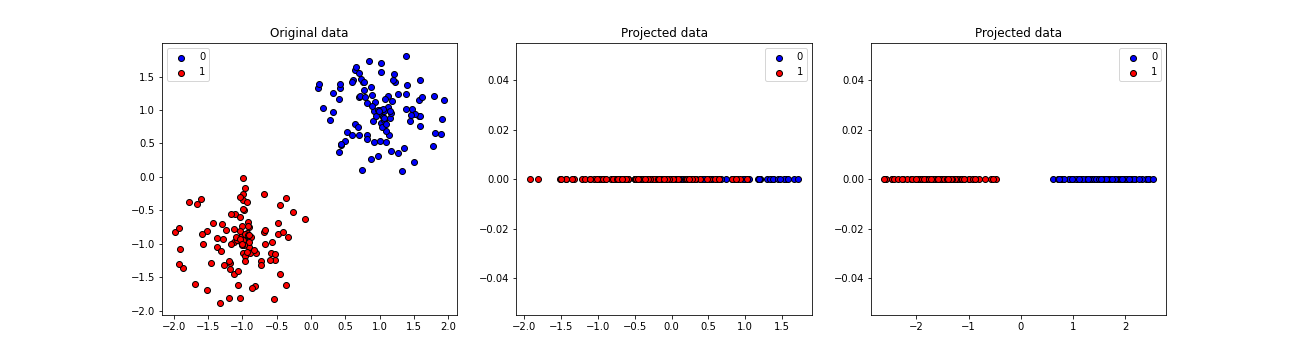
\includegraphics[width=\textwidth]{thesis/Figures/random_projections_example.png}
        \caption{Examples of the random projection invariant.}
    \end{figure}
\end{frame}

\begin{frame}{Random hyperplanes (I)}
    \begin{itemize}
        \item<1-> Based on the \alert{zeroth order invariant}.
        \item<2-> Split the data using a hyperplane passing through one of the
        points of the sample.
        \item<3-> The elements that fall on the right side of the hyperplane will be considered
        as the positive samples, whereas the ones on the left as the negative ones.
        \item<4-> Preserve the proportion of elements of the positive class that fall on the
        right side of the hyperplane.
        \item<5-> Mathematically, this can be expressed as:
    \end{itemize}
    
    \only<5>{
        \begin{equation*}
            \psi_{r.h.}(x) =
            \begin{cases}
                1 & \text{if $(x - x_c)n \geq 0$ }\\
                0 & \text{otherwise}
            \end{cases}
        \end{equation*}
    }
    
    \only<6>{
        \begin{equation*}
            \psi_{r.h.}(x) =
            \begin{cases}
                1 & \text{if $(x - \eqnmarkbox[NavyBlue]{center}{x_c})n \geq 0$ }\\
                0 & \text{otherwise}
            \end{cases}
        \end{equation*}
        \annotate[yshift=1em]{left}{center}{$x_c \in X$}
    }
    
    \onslide<7->{
        \begin{equation*}
            \psi_{r.h.}(x) =
            \begin{cases}
                1 & \text{if $(x - \eqnmarkbox[NavyBlue]{center}{x_c})\eqnmarkbox[WildStrawberry]{normal}{n} \geq 0$ }\\
                0 & \text{otherwise}
            \end{cases}
        \end{equation*}
        \annotate[yshift=1em]{left}{center}{$x_c \in X$}
        \annotate[yshift=1em]{right}{normal}{$n \sim \mathcal{N}(\mu, \Sigma)$, normal vector}
    }
\end{frame}

\begin{frame}{Random hyperplanes (II)}
    \begin{figure}
        \centering
        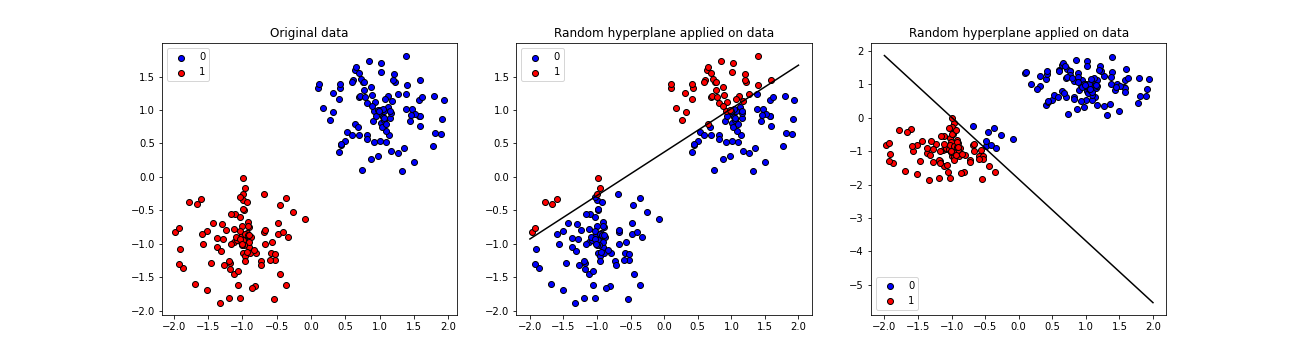
\includegraphics[width=\textwidth]{thesis/Figures/random_hyperplanes_example.png}
        \caption{Examples of the random hyperplane invariant.}
    \end{figure}
\end{frame}

\begin{frame}{Considerations}
    The original LUSI algorithm has to be modified to take into account the stochastic nature
    of these new invariants. Specifically, the following changes have to be introduced:
    
    \begin{enumerate}
        \item<2-> Generate new invariants at each iteration.
        \item<3-> Allow the algorithm to try new invariants when no invariant is selected.
        \item<4-> Limit the number of tries so that the algorithm does not end up in an infinite loop.
    \end{enumerate}
\end{frame}

\begin{frame}{Extending LUSI with ECOC (I)}
    \begin{itemize}
        \item<1-> In order to deal with both the negative class and multiclass classification
        problems, we can extend LUSI using the Error Correcting Output Codes (ECOC) framework.
        \item<2-> The ECOC framework is used to transform multiclass classification problems
        into binary ones.
        \item<3-> For each one of the $N_c$ classes we create a codeword of length $n$. These
        codewords are organized as the rows of a matrix $M \in \set{0, 1}^{N_c \times n}$ called
        the \alert{coding matrix}.
        \item<4-> Each column of the matrix is treated as an individual classification problem
        and a binary classifier is fit with the transformed data.
    \end{itemize}
\end{frame}

\begin{frame}{Extending LUSI with ECOC (II)}
    \begin{table}[!htb]
        \begin{minipage}{.5\textwidth}
            \centering
            \begin{tabular}{c|ccccc}
                            & $h_1$ & $h_2$ & $h_3$ & $h_4$ & $h_5$ \\ \hline
                \textbf{C1} & 1     & 0     & 0     & 0     & 0     \\
                \textbf{C2} & 0     & 1     & 0     & 0     & 0     \\
                \textbf{C3} & 0     & 0     & 1     & 0     & 0     \\
                \textbf{C4} & 0     & 0     & 0     & 1     & 0     \\
                \textbf{C5} & 0     & 0     & 0     & 0     & 1    
            \end{tabular}
        \end{minipage}%
        \begin{minipage}{.5\textwidth}
            \centering
            \begin{tabular}{c|ccccc}
                            & $h_1$ & $h_2$ & $h_3$ & $h_4$ & $h_5$ \\ \hline
                \textbf{C1} & 1     & 1     & 1     & 0     & 0     \\
                \textbf{C2} & 0     & 1     & 1     & 0     & 1     \\
                \textbf{C3} & 1     & 0     & 0     & 1     & 0     \\
                \textbf{C4} & 0     & 1     & 0     & 1     & 0     \\
                \textbf{C5} & 0     & 0     & 1     & 0     & 1    
            \end{tabular}
        \end{minipage}
        \caption{Two examples of coding matrices. The left one represents a special coding called
        one-against-all.}
    \end{table}
\end{frame}

\begin{frame}{Extending LUSI with ECOC (III)}
    \onslide<1-> Let  $f(x) = (f_1(x), \dots, f_n(x))$ be the vector containing the predictions
    for each one of the problems. In order to obtain the final output class, we have to decode
    this vector, which can be done using the following expression:
    
    \vspace{1.5em}
    
    \only<1>{
        \begin{equation*}
            \hat{y} = \argmin_r d(M_r, f(x))
        \end{equation*}
    }
    
    \only<2>{
        \begin{equation*}
            \hat{y} = \argmin_r \eqnmarkbox[NavyBlue]{distance}{d}(M_r, f(x))
        \end{equation*}
        \annotate[yshift=1em]{left}{distance}{distance metric (Hamming, Euclidean, etc.)}
    }
    \onslide<3->{
        \begin{equation*}
            \hat{y} = \argmin_r \eqnmarkbox[NavyBlue]{distance}{d}(\eqnmarkbox[Dandelion]{row}{M_r}, f(x))
        \end{equation*}
        \annotate[yshift=1em]{left}{distance}{distance metric (Hamming, Euclidean, etc.)}
        \annotate[yshift=-1em]{right, below}{row}{$r-$th row of $M$}
    }
    
    \vspace{1.5em}
    
    \onslide<4-> We can use a vector of predicted probabilities and the Euclidean distance.
\end{frame}

\section{Experimentation and results}

\begin{frame}{Overview}
    \onslide<1-> Experimentation with two types of datasets with different goals in mind:
    \begin{itemize}
        \item<2-> Toy datasets
        \begin{itemize}
            \item<3-> Compare the different invariants.
            \item<4-> Compare the original algorithm with the ECOC version.
            \item<5-> Find interesting properties of the invariants.
        \end{itemize}
        \item<6-> Real datasets
            \begin{itemize}
                \item<7-> Assess the quality of the proposed invariants.
            \end{itemize}
    \end{itemize}
\end{frame}

\begin{frame}{Experimentation with toy datasets}
    Compare Vapnik's invariants (zeroth and first order) with random projections and random
    hyperplanes on the Circles and Moons datasets.
    
    \begin{figure}
        \centering
        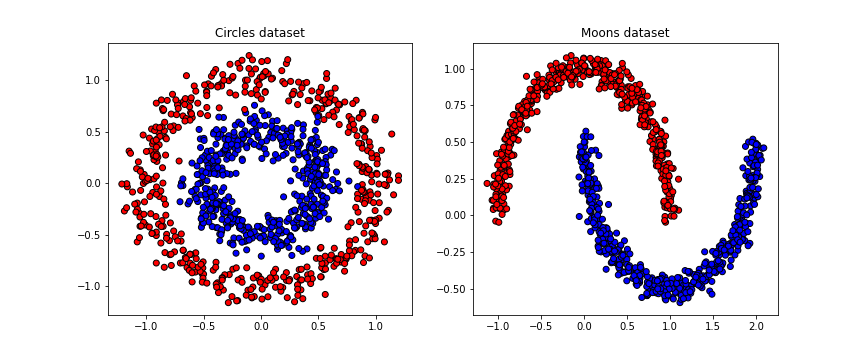
\includegraphics[width=\textwidth]{presentation/figures/toy_datasets.png}
    \end{figure}
\end{frame}

\begin{frame}{Comparing LUSI with the ECOC version (I)}
    \begin{figure}
        \centering
        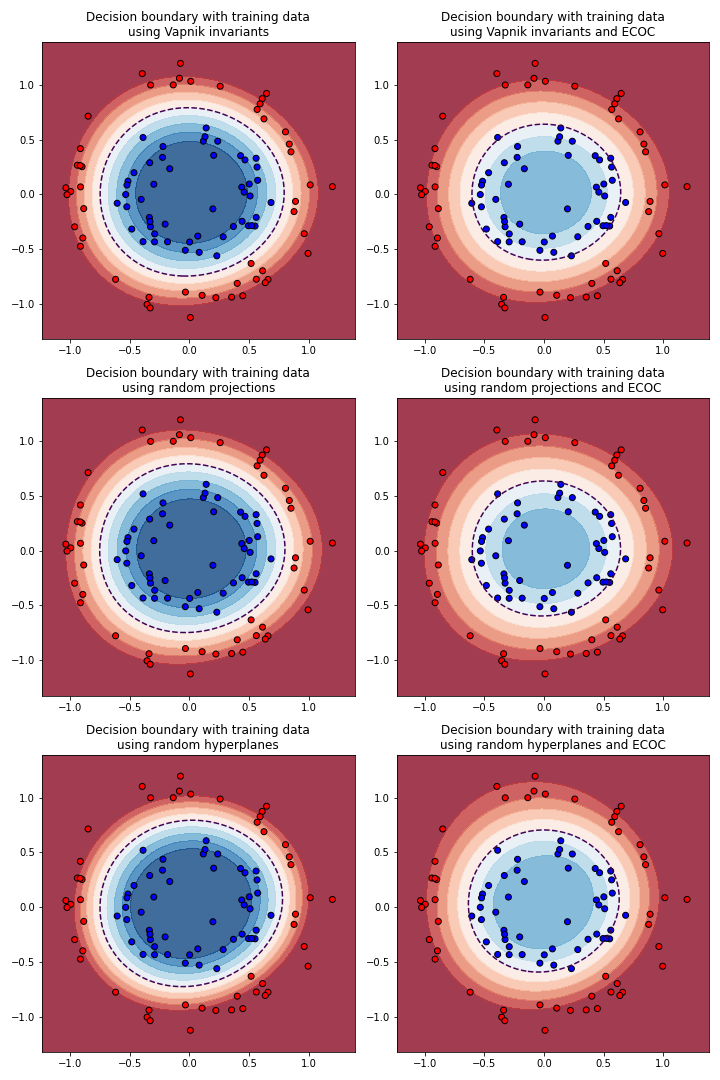
\includegraphics[width=.5\textwidth]{presentation/figures/comparative_circles.png}
    \end{figure}
\end{frame}

\begin{frame}{Comparing LUSI with the ECOC version (II)}
    \begin{figure}
        \centering
        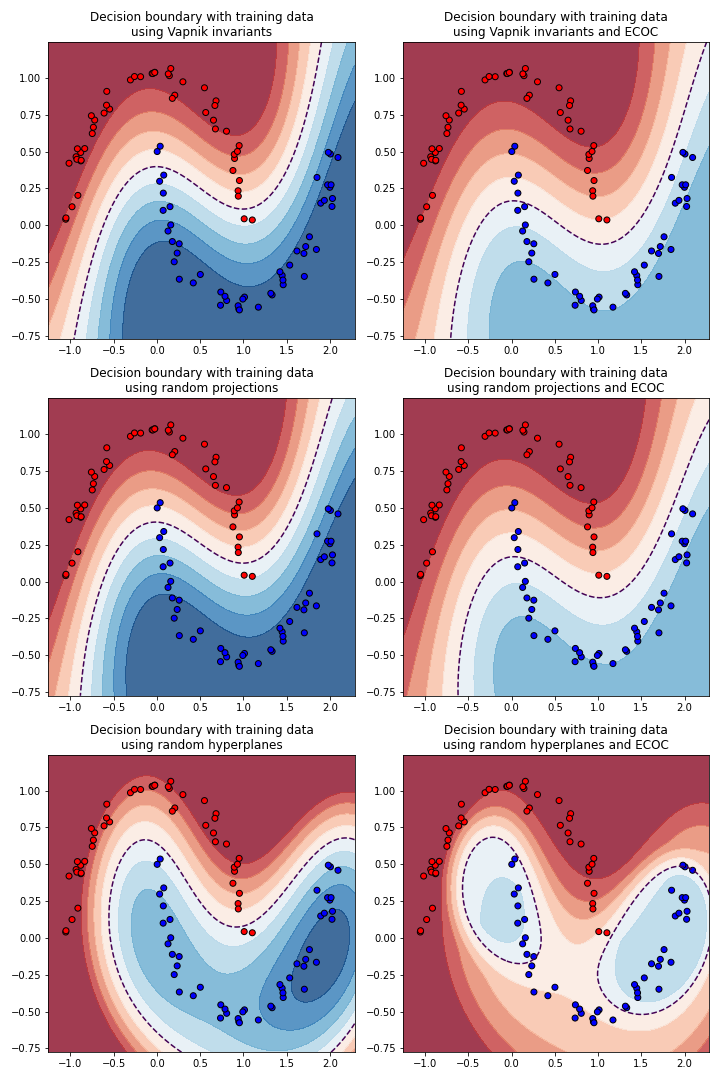
\includegraphics[width=.5\textwidth]{presentation/figures/comparative_moons.png}
    \end{figure}
\end{frame}

\begin{frame}{Comparing the number of selected invariants}
    \begin{figure}
        \centering
        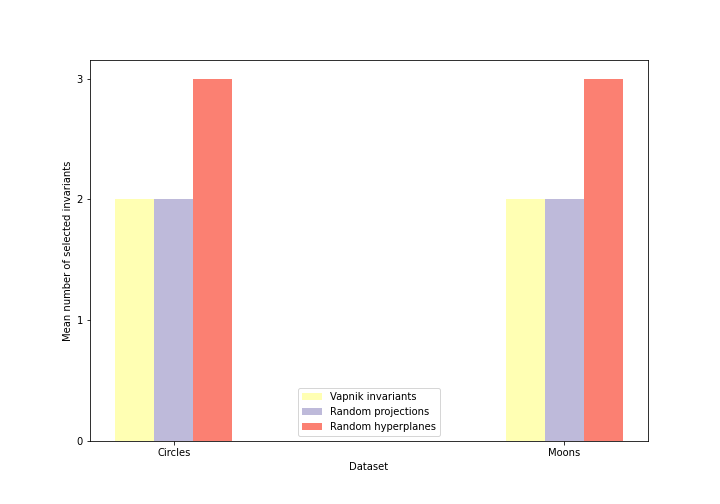
\includegraphics[width=\textwidth]{thesis/Figures/num_selected_invariants.png}
    \end{figure}
\end{frame}

\begin{frame}{Exploring the bias towards certain types of invariants}
    \begin{figure}
        \centering
        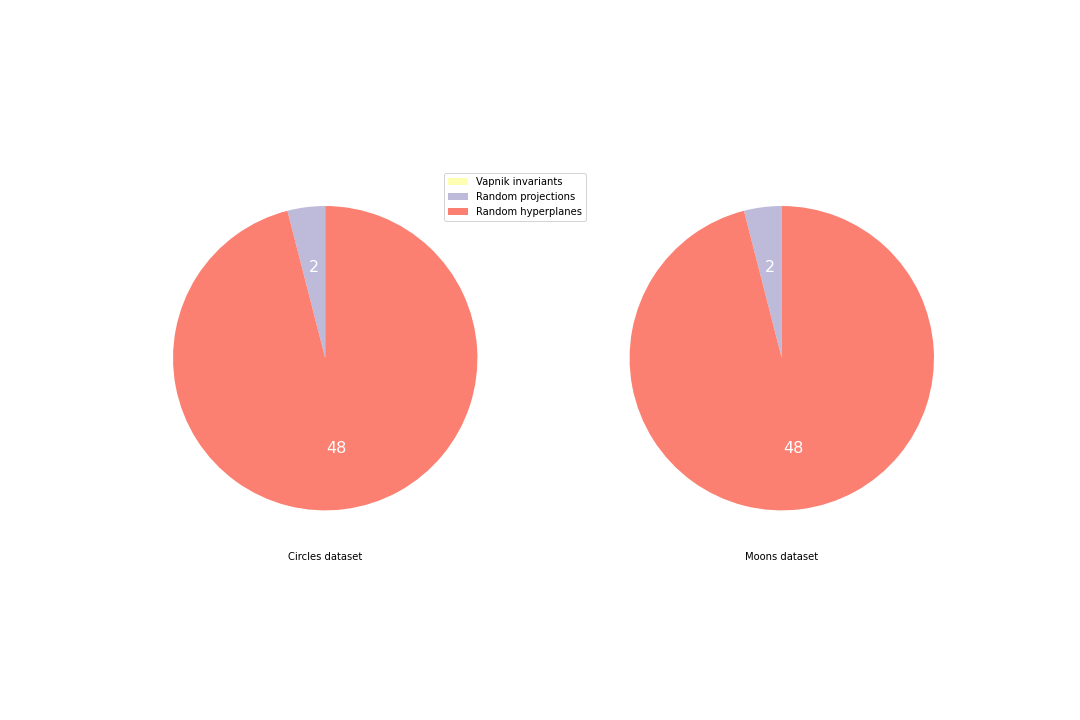
\includegraphics[width=\textwidth]{thesis/Figures/mean_num_selected.png}
    \end{figure}
\end{frame}

\begin{frame}{Experimentation with real datasets}
    \begin{itemize}
        \item<1-> Assess the quality of the invariants on 5 multiclass classification problems.
        \item<2-> Compare 4 models using different types of invariants: no invariants,
        Vapnik's invariants, random projections and random hyperplanes.
        \item<3-> Evaluate the models using different problem sizes: 100\%, 50\% and 10\% of the
        training data.
    \end{itemize}
\end{frame}


\begin{frame}{Selected datasets}

\begin{table}[H]
\centering
\begin{tabular}{lrrr}
\textbf{Problem} & \textbf{Num. examples} & \textbf{Attributes} & \textbf{Classes} \\ \hline
Balance Scale    & 625                    & 4                   & 3                \\
Ecoli            & 336                    & 8                   & 8                \\
Glass            & 214                    & 9                   & \textcolor{red}{6} \\
Iris             & 150                    & 4                   & 3                \\
Yeast            & 1484                   & 8                   & 10              
\end{tabular}
\end{table}
    
\end{frame}

% \begin{frame}{Experimentation methodology}
%     \begin{figure}
%         \centering
%         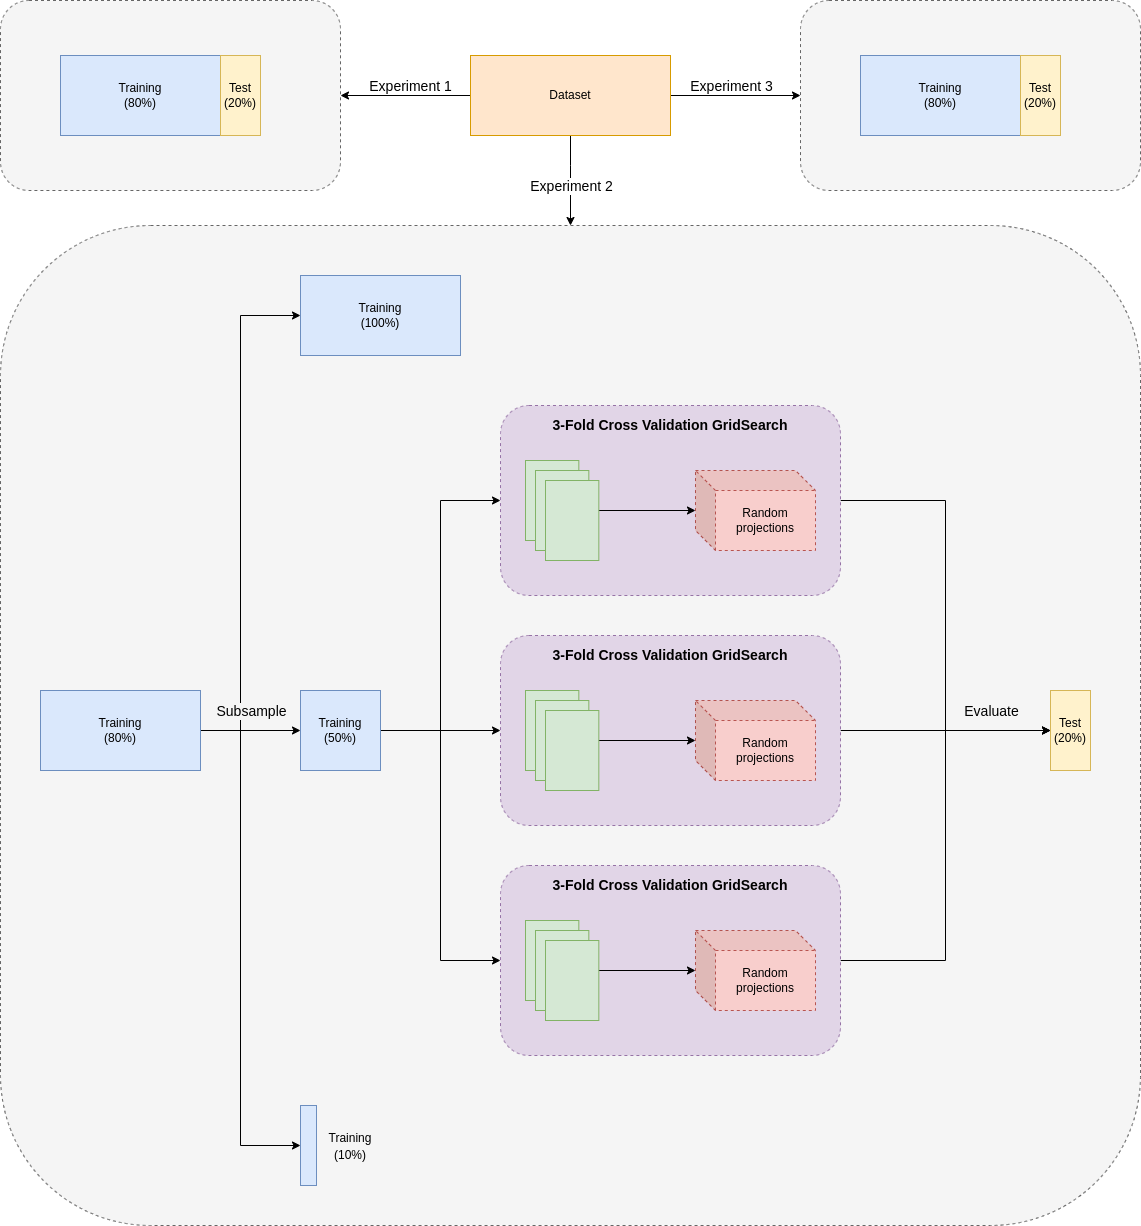
\includegraphics[width=0.7\textwidth]{thesis/Figures/experimentation_scheme.drawio.png}
%         \caption{Caption}
%     \end{figure}
% \end{frame}

\begin{frame}{Results}
\begin{table}
\centering
\resizebox{\textwidth}{!}{%
\begin{tabular}{lcccc}
\textbf{Dataset} & \textbf{Baseline model} & \textbf{Vapnik invariants} & \textbf{Random projections} & \textbf{Random hyperplanes} \\ \hline
Balance Scale & $91.47 \pm 0.38\%$ & $91.47 \pm 0.38\%$ & $\mathbf{91.73 \pm 0.38\%}$ & $90.13 \pm 1.51\%$  \\
Ecoli         & $85.29 \pm 2.08\%$ & $\mathbf{85.29 \pm 1.20\%}$ & $84.15 \pm 2.05\%$ & $75.98 \pm 6.28\%$  \\
Glass         & $\mathbf{72.87 \pm 7.91\%}$ & $\mathbf{72.87 \pm 7.91\%}$ & $72.09 \pm 7.44\%$ & $71.06 \pm 7.60\%$  \\
Iris          & $\mathbf{96.67 \pm 0.00\%}$ & $95.56 \pm 1.57\%$ & $95.19 \pm 1.66\%$ & $88.52 \pm 11.56\%$ \\
Yeast         & $53.76 \pm 1.04\%$ & $\mathbf{53.87 \pm 1.20\%}$ & $52.53 \pm 5.44\%$ & $50.39 \pm 5.33\%$ 
\end{tabular}%
}
\caption{Results using 100\% of the training data.}
\end{table}

\begin{table}
\centering
\resizebox{\textwidth}{!}$ & $87.73 \pm 2.10\%$ & $83.73 \pm 7.17\%$  & $76.00 \pm 12.77\%$ \\
Ecoli         & $71.57 \pm 1.39\%$ & $\mathbf{72.55 \pm 4.22\%}$ & $67.32 \pm 4.03\%$  & $63.89 \pm 9.61\%$  \\
Glass         & $\mathbf{56.59 \pm 4.78\%}$ & $45.74 \pm 6.67\%$ & $52.45 \pm 7.03\%$  & $45.48 \pm 9.50\%$  \\
Iris          & $\mathbf{93.33 \pm 2.72\%}$ & $90.00 \pm 4.71\%$ & $77.78 \pm 22.93\%$ & $84.81 \pm 9.04\%$  \\
Yeast         & $\mathbf{47.92 \pm 2.08\%}$ & $47.92 \pm 2.14\%$ & $45.68 \pm 4.60\%$  & $37.82 \pm 7.92\%$ 
\end{tabular}%
}
\caption{Results using a subsample of 10\% of the training data.}
\end{table}
\end{frame}

\begin{frame}{Comparing the invariants on individual problems (I)}
    \begin{figure}
        \centering
        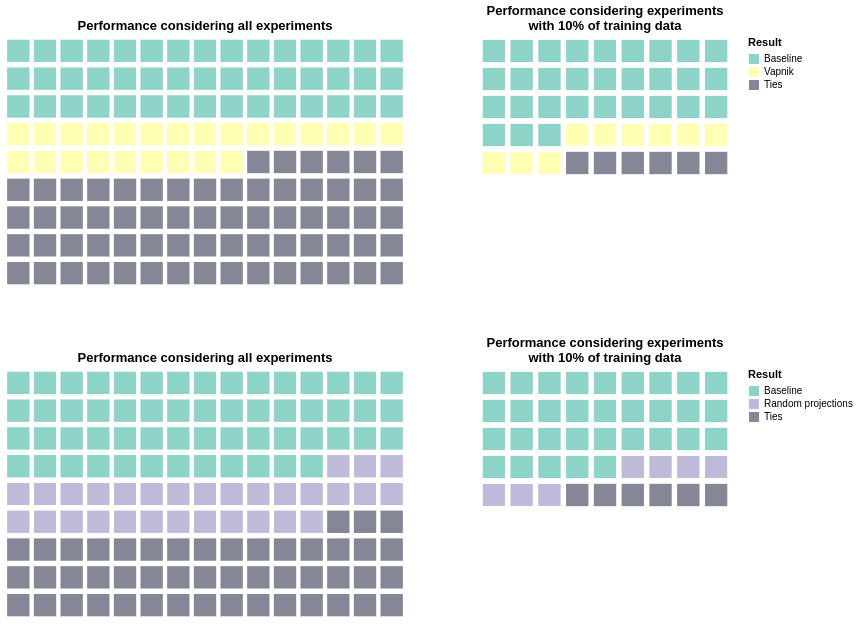
\includegraphics[width=\textwidth]{presentation/figures/invariants_performance_1.png}
    \end{figure}
\end{frame}

\begin{frame}{Comparing the invariants on individual problems (II)}
    \begin{figure}
        \centering
        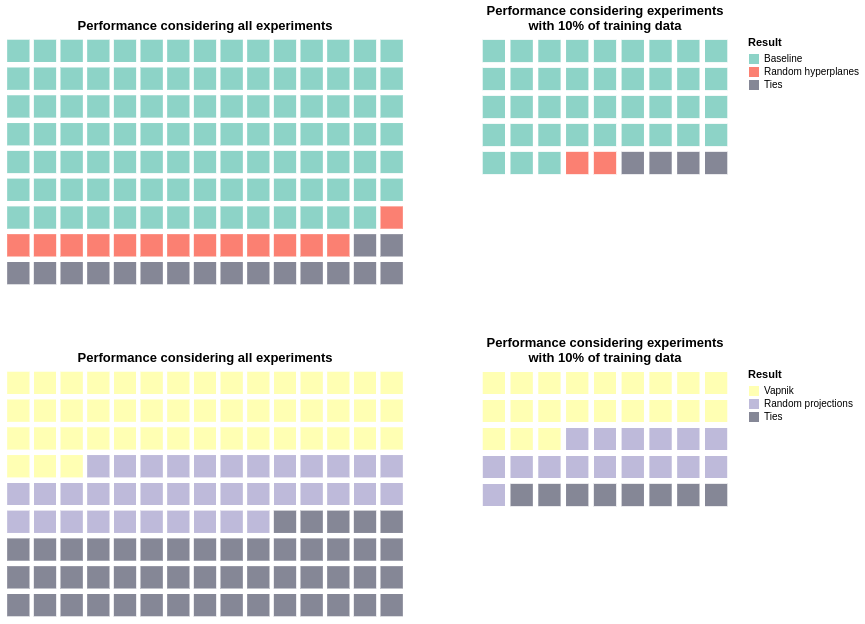
\includegraphics[width=\textwidth]{presentation/figures/invariants_performance_2.png}
    \end{figure}
\end{frame}

\begin{frame}{Comparing the invariants on individual problems (III)}
    \begin{figure}
        \centering
        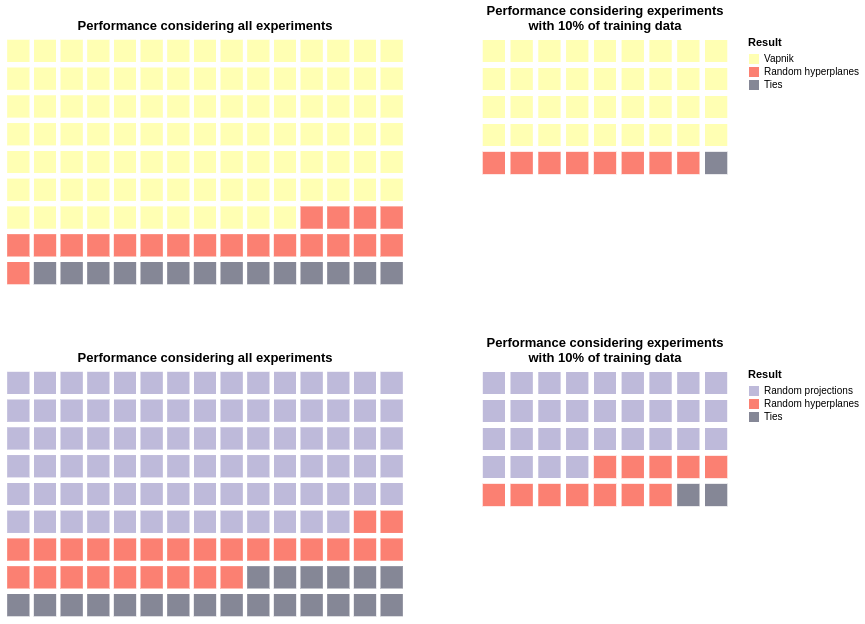
\includegraphics[width=\textwidth]{presentation/figures/invariants_performance_3.png}
    \end{figure}
\end{frame}

\section{Conclusions}

\begin{frame}{Conclusions}
    \begin{itemize}
        \item[\textcolor{Dandelion}{\checkmark}]<+-> Propose new general use invariants that require no prior
        knowledge of the problem.
        \begin{itemize}
            \item<+-> Random projections are slightly worse than Vapnik's invariants.
            \item<+-> Random hyperplanes are outperformed by all the other types of invariants.
        \end{itemize}
        \item[\textcolor{Red}{\XSolidBrush}]<+-> Automatized the selection process of the most suitable
        invariants for a given problem.
        \item[\textcolor{Green}{\checkmark}]<+-> Extend the learning paradigm to multiclass classification problems.
        \begin{itemize}
            \item<+-> Created a small software module containing the different invariants and both the original
            and ECOC version of LUSI.
        \end{itemize}
    \end{itemize}
\end{frame}

\begin{frame}{Future work}
    \begin{itemize}
        \item<1-> Reformulate the optimization problem so that it can be solved by using an iterative
        algorithm.
        \item<2-> Explore higher order invariants.
        \item<3-> Explore invariants for other application domains (images, text, etc.).
        \item<4-> Improve random projections by constructing an orthogonal space from random vectors.
    \end{itemize}
\end{frame}

\begin{frame}[standout]
    Thank you for your attention!
    \rule[-1ex]{\textwidth}{1.5pt}\\[3.5ex]
    Questions?
\end{frame}


\end{document}
